\section{Analysis of \sse Output}\label{sec:ana}

Each execution of \sse creates a folder for analysis output.
Apart from the general log files, where all plugins write important messages, some plugins also create separate files.
For instance one file contains performance characteristics of the test run, another one LLVM bytecode of all analysed programs.
The exact numbers and types of output files depend on which plugins are defined in \sse's configuration Lua script.

The most important information about \sse's general execution is accumulated in \textit{messages.txt}.
Backbone of this file is information about all execution paths, at which memory addresses they were forked, how they are constrained, when and why they were terminated, and much more.
%But it is also used by other plugins...

Thanks to the clear structure of \textit{messages.txt} it can be used as input for a custom Python script. This script was written in order to visualise the tree of execution paths graphically, which serves as a great help with understanding path forking behaviour.
Figure \ref{fig:tree} shows the vital part of the tree of execution paths of \app.

Each box represents an execution state, lines pointing to another state symbolise a fork of the execution state.
The hexadecimal number at the origin of each edge is the memory address in which the state was forked.
For the sake of clarity I also manually added the function in which each memory address occurs.

Edges are labelled with constraints that need to be respected in the corresponding execution state.
KLEE handles constraints in Extended Backus-Naur Form syntax (e.g., ``(Not (Slt (w32 0x20a1) (ReadLSB w32 0x0 v0\_income\_0)))'' for ``income >= 8353'').
For simplicity all constraints were also manipulated manually and transformed into a more readable format.

%Blue state boxes indicate one connection to the internet so far, yellow two and red three.
The text below each leaf shows the output of the \textit{TestCaseGenerator} plugin for this execution path.
Upon termination of a state it finds concrete input examples for the two symbolic variables $income$ and $taxcat$.

\bigskip

Explain!!!!!\todo{!}

\bigskip

Concrete test runs in \sse quickly revealed several \textbf{problems}:

\medskip
1.) Even several hours of execution did not suffice to complete the analysis process.
Every execution had to be terminated prematurely.
Hence analysis output (list of states, etc.) was never complete.
Probable causes of this problem are the following: 
\begin{itemize}
\item Most importantly, the general path explosion as explained in the theoretical part of this paper.
\item Following many execution paths that are irrelevant to the analysis objectives.
\item Execution of \sse on a ordinary laptop and not on a powerful server.
\item Slow communication of the analysed application with a server which simultaneously ran inside the same virtual machine.
\item Inefficient configuration of \sse. Much unnecessary debug and log output, ...
\end{itemize}
The longest analysis run was terminated manually after about six hours.
It pursued over 1000 execution states.
This run produced 164 MB of analysis output, the important pure text file logs being 18 MB big.

\medskip
2.) Due to the extreme duration of analysis runs the original idea to treat all user input as symbolic had to be dismissed. Instead, only two variables ($income$ and $taxcat$) are made symbolic now.
This may be seen as minor cheating since I knew which variables would turn out to be relevant.
A realistic setting will potentially require to run the same analysis with all possible combinations of symbolic variables in order to find a good set of symbolic variables which lead to meaningful analysis results.

\medskip
3.) The initial idea to pursue states in a depth-first search manner turned out to be unwise.
The parts of the execution tree which are vital for a grasp of the program under analysis tend to be close to the root of the tree.
Keeping in mind that all \sse runs had to be terminated prematurely, conducting a depth-first search reveals a multitude of extremely specialised branches and corner cases while neglecting fundamental paths of the tree.

\medskip
4.) The problem of incomplete test results also entailed complications while constructing the execution tree, which of course never was consistent.
For this reason and due to the fact that most states are irrelevant for the goals in this paper anyway, the tree in figure \ref{fig:tree} shows a radically trimmed version of the original execution tree.

%4.) Baum muss auch getrimmt werden, weil die allerallermeisten Forks Müll sind.


%It is only the root because....
%The whole graph (without constraints) looks as folllows:...

\begin{figure*}
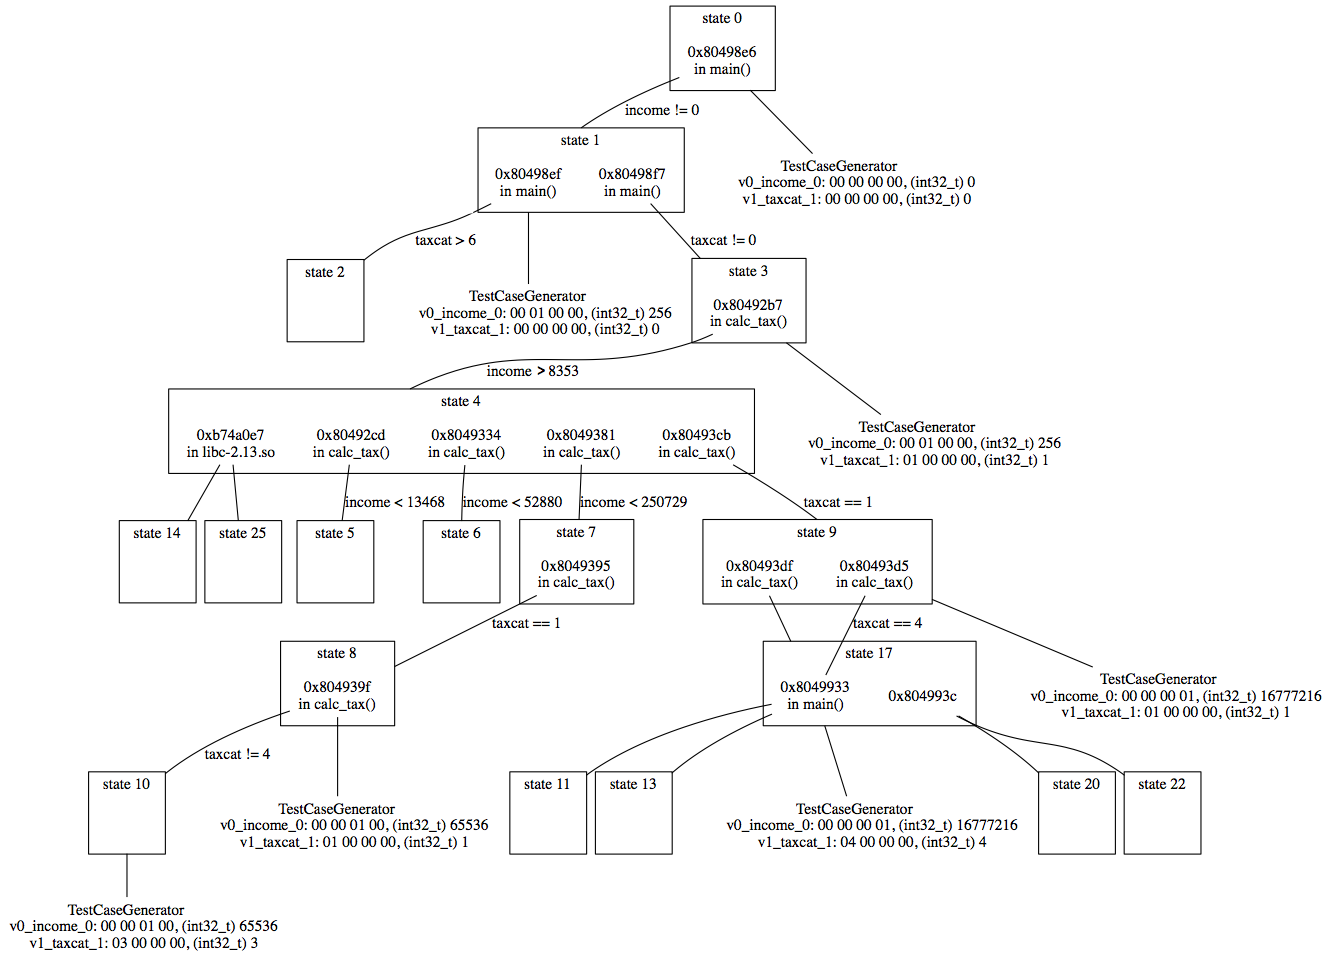
\includegraphics[width=\textwidth]{cool3}
\caption{Tree visualisation for understanding path forking behaviour in the analysis of \app. Shows at which memory addresses \sse forked new execution states. Path constraints are printed at each state transition. For most states, the \textit{TestCaseGenerator} found meaningful concrete example values for the two symbolic variables $income$ and $taxcat$.}
\label{fig:tree}
\end{figure*}



\iffalse
§6	Interpretation of S2E analysis output
		> Execution Traces
		> Gefundene Privacy-Probleme
		> Eventuell nicht gefundene Sachen
		> Probleme bei der Analyse
\fi